\chapter{Domän - problembeskrivning och analys}
I detta kapitel beskrivs centrala frågeställningar som rör  modellering av domänen och andra icke-tekniska ämnen.

\section{Inlämningskanaler}

Det nya systemet ska vara anpassat för användare med olika kunskapsnivåer. En konsekvens av detta är att inlämning via versionshanteringsklient inte kan vara det enda tillvägagångssättet. Studenter vid olika program och vid olika skeden av sin utbildning kan ha varierad eller ingen erfarenhet av versionhantering. Det är därför viktigt att erbjuda flera kanaler.

\subsection{Git}
Git som inlämningskanal behandlas i  [HÄNVISNING TILL AVSNITT].

\subsection{Webbgränssnitt}
Uppladdning genom webbgränssnitt är den lösning som används i Fire. Metoden är robust och bekant för de flesta. Projektgruppen anser dock att lösningen lider av ett antal begränsningar. Det enda sättet att ladda upp flera filer på samma gång är med arkivfiler i tar.gz-format (Gedell, T. (2006), Upload File). Detta är också det enda tillgängliga sättet att ladda upp mappstrukturer. Det går heller inte att bläddra i innehållet i filer eller tar.gz-arkiv, vilket leder till att studenter ofta känner sig tvungna att ladda ner en hel inlämning igen för att känna sig säkra på att innehållet är korrekt.

Water bör erbjuda ett mer flexibelt sätt att ladda upp filer. Uppladdning av flera filer på samma gång bör vara möjligt. Det bör också gå att skapa mappar och ladda upp filer till olika ställen i en mappstruktur. För att detta ska vara möjligt bör Water möjliggöra navigering i filstrukturer.

\subsection{E-post}
Ytterligare en potentiell metod för inlämning är via e-post. Studenter skulle då kunna skicka in inlämningar som bifogade filer. För att knyta en inlämning till en specifik uppgift inom en viss kurs så skulle systemet kunna generera unika identifikationskoder som studenten skickar med i mailet. Förslagsvis skulle man vid registrering för en kurs i systemet få ett mail per uppgift som innehåller all information som behövs för att kunna utföra laborationen. Studenten skulle då kunna lämna in till en specifik uppgift genom att svara på mailet som är knutet till den uppgiften.

Som vi såg det skulle logiken för mailinlämningar riskera att bli väldigt invecklad. Om syftet med att utöka antalet inlämningskanaler är att höja användarvänligheten, så finns det ingen anledning att lägga till en kanal där inlämningsförfarandet är onödigt komplicerat.

\begin{flushright}
  \textbf{Beslut}
  
  Inlämningskanalerna begränsas till versionshanterare och webbgränssnitt för att undvika komplexiteten i att implementera inlämning via e-post.
\end{flushright}


\section{Frågor gällande inlämning via versionshantering}\label{sec:fragor-git}
I systemet behövs lämpliga sätt att relatera koncept inom versionhantering till inlämningsuppgifter. Frågan kan delas upp i två delar: hur inlämningarna ska förvaras och hur inlämningen sker.

\subsection{Förvaring av inlämningsuppgifterna}
Vad gäller förvaringen ser kandidatgruppen två alternativ:

Antingen skapas ett nytt repositorium för varje grupp och inlämningsuppgift, eller så sparas gruppens samtliga inlämningsuppgifter i ett repositorium, men i olika grenar.

I skarpa projekt har varje delprojekt ett eget repositorium. Särskilt vanligt är detta för distribuerade versionhanteringssystem, eftersom de ofta inte erbjuder clone för bara delar av ett repositorium. Se till exempel Git (git-clone(1) Manual Page, 2012). Kandidatgruppen är av uppfattningen att \emph{branches} traditionellt uppfattas som olika versioner av samma kodbas. Detta stöder idén om att använda ett repositorium per inlämningsuppgift. Det leder även till separation mellan inlämningsuppgifter – misstag eller tekniska problem inom en inlämningsuppgift inte drabbar andra inlämningsuppgifter. Metoden öppnar även för att Water i framtiden erbjuder studenterna flera \emph{branches} att arbeta med, till exempel för att definiera delmoment i inlämningsuppgifter eller som ett kollaborationsverktyg.

En nackdel med separata repositorier är att det krävs en \emph{remote-url} per repositorium, och därmed per inlämningsuppgift. För varje inlämningsuppgift måste studenten hämta en \emph{remote-url} ifrån webbapplikationen och använda den för att konfigurera sin versionshanterare.

\subsection{Inlämning via versionshantering}
Vad gäller själva inlämningen finns ett antal tänkbara strategier.

En möjlighet är att låta varje commit utgöra en inlämning. Metoden är lätt att implementera, men tillåter inte att studenterna bygger upp en inlämning med hjälp av ett antal commits och bidrar heller inte till kollaborering.

En annan möjlighet är att använda taggar. Taggar är ett sätt att knyta metadata till ett visst tillstånd i versionshanteringsträdet. Taggar kräver dock ofta att användaren lär sig en speciell syntax. I Git, exempelvis, krävs dessutom att användaren uttryckligen begär att taggar ska skickas med när ändringar överförs via en push till en annan nod.

Ett alternativ till taggar är att definiera speciella strängar som användaren kan skriva in i commit-meddelandet. Versionshanterar-servern analyserar alla inkommande commits för att leta efter dessa. Denna metod används bland annat av code hosting-tjänsten Github för att göra det möjligt att knyta en commit till en issue i deras issuehanteringssystem. Där räcker det med att skriva \#1 för att referera till issue nummer 1. Water skulle kunna lyssna efter en lämplig sträng som signalerar att commiten i fråga ska utgöra en inlämning.

\begin{flushright}
  
  \textbf{Beslut}
  
  För varje inlämningsuppgift har en grupp ett repositorium. I systemet definieras en \emph{branch} som global inlämningsbranch. I vårt fall är det master som används för inlämningar. Inlämningar kan konstrueras som ett antal commits, själva inlämningen sker genom att commit-meddelanden innehåller strängen \#submit.
\end{flushright}

\section{Inlämningens livscykel}

Grundantagandet i Water är att en inlämning i sin enklaste form är en pekare till ett visst tillstånd i ett repositorium – en commit. Inlämningen går igenom ett antal tillstånd innan uppgiften kan godkännas. När denna livscykel ska utformas ställs krav som enkelhet, flexibilitet och tydlighet mot varandra.

\subsection{När ska inlämningskanalerna öppnas och stängas?}
Grundidén är att inlämningskanalerna stängs när deadline passerat eller när en inlämning har gjorts för att undvika att rättaren arbetar med en inlämning som inte längre är aktuell. Kanalerna öppnas igen om inlämningen är underkänd.

Ur studenternas perspektiv är det dock önskvärt att kunna göra ändringar i en inlämning så länge som möjligt. En typisk situation är att filer fattas eller att något uppenbart fel uppdagas efter att inlämning har skett. Det förefaller onödigt att låta studenterna vänta på att en rättare underkänner inlämningen innan de kan rätta felet.

En kompromiss är att tillåta ändringar i en inlämning tills rättaren har börjat arbeta med den. 

\subsection{Uppdatering av inlämningar}
Teoretiskt vore det möjligt att se ändringar av inlämningar som nya inlämningar. I så fall skulle studenterna ha rätt att göra ett obegränsat antal inlämningar tills dess att rättaren inleder sitt arbete. Detta leder dock till att det kan finnas föräldralösa inlämningar i systemet som aldrig kommer att behandlas, vilket gör hanteringen av dem svårare.

För att undvika detta är det möjligt att se ändringar i inlämningar som uppdatering av en befintlig inlämning. Vid uppdatering riktas pekaren i inlämningen till ett nytt tillstånd i inlämningsrepositoriet. Det öppnar även för enklare hantering av till exempel deadlines, eftersom till exempel den första deadlinen kan relateras direkt till den första inlämningen.

\subsection{När inlämningen har rättats}
Om en inlämning blir godkänd bör det inte längre vara möjligt att lämna in fler inlämningar. Om inlämningen däremot är icke-godkänd, och chans för ytterligare inlämning finns, bör inlämningskanalerna öppnas igen.

\begin{flushright}

  \textbf{Beslut}

  En inlämning kan uppdateras så att den pekar på ett nytt tillstånd i ett repositorium tills handledaren har börjat rätta den. Blir inlämningen underkänd kan en ny inlämning skapas. Blir inlämningen godkänd är det inte längre möjligt att lämna in.
\end{flushright}

\section{Tillståndshantering - vilken entitet är det som blir godkänd?}

För att implementera inlämningens livscykel behövs ett antal tillstånd och strategier för att hantera de olika stegen.

För betygssättning behövs tillstånd för godkända och underkända inlämningar. För att kunna implementera uppdatering av inlämningar, vilket behandlas i avsnitt \ref{sec:uppdatering-inlamningar}, behövs skilda tillstånd för inlämningar som väntar på bearbetning av handledare och inlämningar där arbetet har inletts.

Vid första anblick är det oklart vilken entitet i modellen som ska hantera dessa tillstånd. Tydligt är dock att handledarna i första hand kommer att behandla inlämningar för att kunna sätta ett betyg på en inlämningsuppgift. Den naiva lösningen är alltså att låta inlämningsentiteterna hantera tillstånd.

Det är på samma gång tydligt att det är grupper som får hela inlämningsuppgifter godkända, vilket talar för att tillståndet istället lagras i en entitet som kopplar grupper till uppgifter.

\subsection{Tillståndshantering i flera entiteter leder till redundans}
Ytterligare en lösning är att placera tillstånden där de tycks passa bäst – både i inlämningentiteten och i entiteten som kopplar grupper till laborationer. Detta skapar dock redundans i modellen eftersom informationen finns tillgänglig även om den bara sparas i den ena entiteten. Till exempel betyder en godkänd inlämning att även laborationen är godkänd. En godkänd laboration betyder att den sista inlämningen är godkänd och de övriga är icke-godkända eller icke rättade, beroende på hur modellen är beskaffad.

Redundans bör undvikas av de anledningar som diskuteras i kapitel \ref{sec:databasen}.

\subsection{Tillståndshantering i endast en entitet kan leda till oklara tillstånd}
Om tillståndshanteringen endast placeras i inlämningsentiteten blir det lätt att hämta information om enskilda inlämningar. Däremot måste alla inlämningsentiteter för en grupp och en inlämningsuppigft hämtas och kontrolleras när systemet ska beräkna hela inlämningsuppgiftens tillstånd.

Om tillståndshanteringen istället placeras i entiteten som kopplar grupper till inlämningsuppgifter är det lätt att hämta information om gruppens tillstånd i förhållande till inlämningsuppgiften. Det kan i gengäld bli svårare att ta reda på tillståndet för en enskild inlämning, beroende på hur modellen är uppbyggd. Problem uppstår om systemet tillåter föräldralösa inlämningar, vilket beskrivs i avsnitt \ref{sec:uppdatering-inlamningar}, och gruppen har gjort två eller flera inlämningar och den sista inlämningen är icke-godkänd. I detta fall är det omöjligt att veta om inlämningarna före den icke-godkända inlämningen är icke-godkända eller föräldralösa. Det går att betrakta alla inlämningar före en icke-godkänd inlämning som icke-godkända, men det leder till att inlämningar som aldrig har behandlats av en handledare ser ut att ha blivit behandlade.

Om systemet inte tillåter föräldralösa inlämningar går det att entydigt bestämma enskilda inlämningars tillstånd utifrån gruppens tillstånd i relation till inlämningsuppgiften.

\begin{flushright}

  \textbf{Beslut}

  Tillstånd hanteras i entiteten LabHasGroup, som beskrivs i modellavsnittet \ref{sec:modell-labhasgroup}. Entiteten representerar grupper i relation till inlämningsuppgifter. Enligt tidigare beslut tillåts inte föräldralösa inlämningar, vilket gör att enskilda inlämningars tillstånd kan entydigt bestämmas.
\end{flushright}

\section{Validering av inlämningar}\label{sec:valideringar}

I laborationer finns i allmänhet krav som måste uppfyllas för att de skall bli godkända. Typiska exempel på detta kan vara att inlämningen skall bestå av filer med speciella namn, ha en viss typ av filformat, maximalt antal tecken i radbredd eller gå igenom de tester som bifogats med laborationsbeskrivningen.

I det nuvarande systemet måste handledare manuellt neka inlämningar som inte uppfyller dessa krav. Handledarna får spendera tid på att avvisa laborationer som inte är giltiga då studenterna har slarvat med innehållet, men kanske har en korrekt lösning. Studenterna i sin tur förlorar ett av sina inlämningsförsök och blir först medvetna om detta efter att handledaren fått tid att titta på den.

En lösning till detta vore att i det nya systemet erbjuda automatiska valideringar vid varje inlämning. Dessa skulle kunna, så fort testerna är klara, meddela studenten om inlämningen uppfyller de grundläggande kraven - så denne får en omedelbar chans att rätta till felaktigheterna. Oftast har studenterna endast ett begränsat antal inlämningar på sig innan en laboration måste vara godkänd. Om en inlämning som inte passerar testerna skall minska antalet kvarvarande försök eller ej är något som skulle behövas ta ställning till.

Vad som skulle ingå i valideringen av en inlämning skulle behöva konfigureras efter specifikationerna för varje laboration. 

\begin{flushright}
  
  \textbf{Beslut}
  
  Möjlighet till valideringar undersöktes under projektet, men implementerades inte. Dock är funktionaliteten högprioriterad vid vidareutveckling av systemet.
  
\end{flushright}
\section{Rättning}

I Fire finns ett antal uppskattade funktioner för handledare. Bland annat kan handledaren ladda ner samtliga inlämningar som den ska rätta i ett tar.gz-arkiv (Gedell 2006b). Funktioner som dessa bör finnas även i Water.

Fire har dock några brister i rättningsfunktionen.

Handledare upplever ibland att det är svårt att se exakt vad som har ändrats mellan två inlämningar\footnote{Intervju med Oskar Utbult den 2 mars 2012}. Genom att som i Water basera inlämningssystemet på versionshantering är det lätt att ta fram skillnaden mellan två tillstånd – en såkallad \emph{diff}. En handledare som använder sig av ett versionshanteringssystem för att hämta inlämningar kan enkelt skapa en \emph{diff} själv. Water bör erbjuda visualisering av \emph{diffar} i webbgränssnittet.

Fire låter användaren hämta rena textfiler via webbgränssnittet, men kan inte hantera mappstrukturer. Studenter som vill lämna in projekt med annat än en endimensionell mappstruktur måste använda arkivfiler för att göra detta. Detta innebär även att handledarna måste ladda ner projekten som arkivfiler, istället för att förhandsgranska den i webgränssnittet.

Många inlämningar vore möjliga att rätta direkt i ett webbgränssnitt om det erbjöd navigering i mappstrukturer och rendering av källkodsfiler. Detta skulle göra handledarnas jobb mer flexibelt. Water bör erbjuda denna funktionalitet.

\begin{flushright}
  
  \textbf{Beslut}
  
  Water erbjuder uppladdning av flera filer på samma gång, bläddring i mappstrukturer, manipulation av mappstrukturer och rendering av källkod. Nedladdning av inlämningar i arkivformat och visning av diffar implementeras inte, men är högprioriterat vid vidareutveckling av systemet.
  
\end{flushright}
\section{Insyn i rättningsprocessen}

Från projektgruppens sida finns det en önskan om större insyn i rättningsprocessen.

En möjlighet är att upprätta ett kösystem. Samtliga inlämningar i hela kursen läggs i en rättningskö där de prioriteras efter vilken uppgift inlämningen gäller, inlämningstid, om inlämningen är svar på en retur och andra liknande faktorer. En ledig handledare skulle vara tvungen att rätta den inlämning som står längst fram i kön, i detta fall skulle studenterna få väldigt exakta uppgifter om sin köplats. Problemet med detta system är att reglerna för kösystemet skulle bli tämligen rigida och att de nödvändigtvis inte skulle passa för alla sorters kurser.

En annan möjlighet är att ge handledarna den information som de behöver för att själva göra prioriteringarna utan att bygga en tvingande kö i systemet. På detta sätt är systemet mer flexibelt men det skulle bli svårt att ge studenterna tydliga indikationer om hur rättningen fortskrider.

En kompromiss är att inlämningarna delas in i mindre prioritetsköer beroende på vilken laboration de hör till. Handledarna väljer vilken laboration de vill rätta, men är bundna till prioritetsköerna för den valda laborationen. 

\begin{flushright}

  \textbf{Beslut}

  Inga rigida prioritetsköer implementeras för rättning. Rättarna får göra prioriteringarna själva. Detta eftersom behoven i olika kurser kan variera på sätt som projektgruppen inte kan förutse.
\end{flushright}

\section{Anonym rättning}

På CTH har anonym rättning införts för alla salstentamina (Chalmers Studentportal, Anonyma tentor). För att förbättra studenternas rättssäkerhet valde kandidatgruppen att utreda om anonym rättning kunde införas även för laborationer.

Fördelar med anonym rättning är att studenter är garanterade en rättvis rättning där rättarens personliga åsikter inte kan påverka resultatet, anonym rättning innebär också att studenter kan argumentera med sina lärare om kursen och dess innehåll utan att oroa sig för negativa effekter vid bedömning.

Ett enkelt sätt att implementera detta på är att ersätta studenternas namn med sifferkoder eller liknande i vyerna. Då är det sparat i databasen vem det är och en administratör kan lämna ut uppgifterna om en elev eller grupp om nödvändigt.

Anonym rättning lämpar sig inte nödvändigtvis för alla sorters laborationer och så länge det inte finns något policybeslut om det från universitetet bör användandet av funktionen vara valbart för var kurs.

\begin{flushright}

  \textbf{Beslut}

  Då anonym rättning inte är en kritisk del av projektet har det blivit nedprioriterat.
Eftersom implementetationen är relativt enkel kommer den här funktionen troligtvis dyka upp i en senare version av mjukvaran.
\end{flushright}

\section{Kommunikation}

Ett syfte med Water är att förbättra kommunikationen mellan studenter och personal. Dessa förbättringar kan ske på olika nivåer.

Ett system som Water skulle kunna användas som allmän informationskanal, till exempel för meddelanden som handlar om kursval och dylikt,  eftersom det har tillgång till samtliga studenter som är registrerade på en kurs. Alla kurser på en institution kommer dock inte att använda Water. Därför är det bättre att använda andra verktyg för allmän kommunikation med studenterna. Fokus i Water ligger istället på att förbättra den kommunikation som sker mellan studenter och handledare i anknytning till inlämningsuppgifter.

\subsection{Kommunikation kring inlämningsuppgifter}
Som tidigare nämnt kan handledare i Fire inkludera kommentarer när de rättar en inlämningsuppgift. Studenterna kan endast svara med en ny inlämning. Studenterna riskerar att missuppfatta återkopplingen, vilket kan leda till att även den korrigerande inlämningen förkastas onödan. För att råda bot på detta vill projektgruppen att Water  ska erbjuda en dialog mellan handledare och student.

Detta kan implementeras genom ett kommentarssystem. Systemet låter handledare kommentera inlämningar. Handledarens kommentarer presenteras sedan tillsammans med koden i webbgränssnittet. Studenterna kan därefter svara på handledarens kommentarer med egna kommentarer.

Ytterligare en möjlighet är att erbjuda så kallade inline-kommentarer, det vill säga kommentarer som är knutna till specifika rader i inlämnade filer. Detta skulle göra det möjligt för handledarna att ge återkoppling på väldigt specifika problem, istället för att försöka referera till dem i löpande text i en kommentar till inlämningen.

Alla parter bör bli underrättade när nya kommentarer har kommit in.

\section{Laborationsgrupper i Water}

Fire möjliggör för studenter att arbeta i nya grupper under varje laboration. I systemet kan en student skapa flera grupper och bjuda in olika personer till var grupp. Vid kursslut förstår Fire huruvida en student avklarat alla laborationer i kursen oavsett i vilken av sina grupper laborationen fullgjorts. Vanligtvis laborerar elever i samma grupp under en  hel kurs men systemet behöver kunna hantera studenter som jobbar i olika grupper i samma kurs.

Laborationsgrupperna i Water kommer att efterlikna funktionaliteten som finns Fire och utvidga den.

\subsection{Avhopp från laborationsgrupper}
Av olika skäl kan det finnas behov av att splittra grupper.  Till exempel kan studenterna ha blivit oense eller avregistrerat sig från kursen. Konceptuellt måste det vara möjligt att dela upp grupper. Den naiva lösningen är att bara radera en grupp och att skapa nya. När en grupp raderas försvinner alla inlämningar den gruppen har gjort då det inte får finnas Git-repositorier som inte tillhör någojen grupp, detta leder också till att informationen som anger vilkaimalt laborationer gruppen har klarat raderas.

\begin{itemize}
  \item En student som avregistrerat sig från en grupp skall ej få godkänt på laborationer som kvarvarande i gruppen lämnar in.
  \item Ingen data skall tas bort vid avhopp, speciellt inte avklarade laborationer.
  \begin{itemize}
    \item Studenternas material måste finnas kvar och vara tillgängligt för dem.
  \end{itemize}
  \item Som en studentanvändare av Water vill man känna sig trygg med att splittringsoperationen inte tar bort något. Till exempel måste inskickade laborationer förbli inskickade och rättas för alla deltagare i den splittrade gruppen. Den splittrade gruppen bör kunna fortsätta arbeta tillsammans vid retur, även om de börjat arbeta i nya grupper. En student skall alltså kunna förstå med hjälp av gränssnittet att ovanstående situation gäller när de splittrar gruppen.
\end{itemize}

Vi presenterar nedan två lösningsideer som gruppen övervägde mellan. I lösningarna tar vi upp perspektiv både på användargränssnitt och databasmodell.

\subsection{Faktisk splittring av grupper}
Ett naturligt sätt att utföra splittringen på är att försöka efterlikna det konceptuella att en eller flera studenter faktiskt hamnar i en ny grupp medan resterande är kvar. För att de nya studenterna ska kunna ha kvar sitt material från sin splittrade grupp krävs det att de avklarade laborationerna kopieras över till deras nyskapade grupp. Att kopiera data i en databas anses som allmänt fel då en \emph{normaliserad} databas, vilket beskrivs djupare i kapitel \ref{sec:databasen}, ska ha minimalt med redundans. Man kan också låta laborationer “ägas” av själva studenterna och inte gruppen. I detta fall kommer en splittrad grupp inte påverka studenternas datatillgång eftersom den inte baseras på grupper.

\subsection{Immuterbara grupper}
En annan lösning är att låsa medlemmarna i en laborationsgrupp, vilket innebär att man inte kan splittra en grupp. Paradigmen blir då att gruppen motsvarar en fixt grupp av studenter. Att på detta sätt ha oföränderliga grupper löser direkt problemet med hur man kopierar över material till nya grupper, eftersom grupper aldrig splittras. Operationen av en konceptuell splittring för en grupp på två studenter kommer utföras genom att båda studenter skapar var sin ny grupp, alternativt går med i redan existerande grupper. Ett till problem som löses med detta är att studenter inte heller kan gå med i en låst grupp, alltså en student som inte utfört en laboration kan inte bara gå med och få godkänt på tidigare laborationer avklarade av den gruppen.

Också denna lösning introducerar problem, nämligen att definiera hur en grupp bildas och populeras med studenter. Om alla grupper börjar frysta skulle en nyskapad grupp förbli tom.

Det är inte självklart att immuterbara grupper är begripligt för en studentanvändare.  Vi vet inte om en grupp elever som vill splittras naturligt tänker sig att de “splittrar” sin grupp eller om de direkt förenklar det till att de skapar varsin ny grupp.

\begin{flushright}

  \textbf{Beslut}

  Vi valde immuterbara grupper för det är enklare då vi egentligen inte behöver implementera splittring av grupper. Immuterbarheten möjliggör även att forcera invarianter för studenters laborationsantal.
\end{flushright}

\section{Invarianter för studenters laborationsantal}

Det finns möjlighet att ha en invariant mellan hur många simultana “laboration-till-grupp”-kopplingar det finns per laboration för varje enskild student. Det rör sig mellan alternativen att forcera maximalt en koppling per laboration, att forcera till exakt en koppling per laboration samt att strunta i att ha invarianten. Det leder till mer arbete att uppehålla en striktare invariant, men det har fler fördelar.

För att göra detta avsnitt läsbart inför vi termen LabHasGroup, förkortad LHG. LHG är den entitet i modellen som representerar kopplingen mellan en grupp och en laboration. [HÄNVISA TILL MODELL-KAPITEL]

\subsection{Max en LHG per laboration ($\leq 1$)}
Som en direkt konsekvens av denna invariant kan inte en student lämna in samma laboration genom flera laboration till grupp kopplingar eftersom invarianten direkt stryper kopplingsantalet till maximalt en per laboration. I praktiken jobbar aldrig en student på samma laboration via flera kopplingar samtidigt. Det är troligt att studentanvändare blir förvirrade av att de ser att de jobbar på samma laboration via olika kopplingar. Det bör alltså noteras att fördelarna är främst  ytliga, alltså att produktens webbinterface blir tydligt för studentanvändarna. Vidare ska en handledare inte av misstag behöva rätta två inlämnade laborationer kopplade till samma student.

Flera möjliga sätt finns för att enforcera invarianten, gemensamt för implementeringssätten är att de måste definera nödvändiga gruppoperationer och visa att de är riskfria, det vill säga att invarianten aldrig bryts efter operationerna har utförts. Några operationer kan tänkas vara följande:

\begin{itemize}
  \item Skapa grupp
  \item Gå med i grupp
  \item Eventuellt “starta laboration”
  \item Ta bort,  inaktivera eller frysa en laboration – dessa operationer är ekvivalenta
\end{itemize} 

Eftersom grupperna är immuterbara finns inte operationerna elevavhopp eller gruppsplittring. Invarianten syftar på antalet aktiva grupper vilket skulle betyda att operationerna: ta bort, inaktivera samt frysa en LHG är alla ekvivalenta vad berör denna invariant.  Att starta en laboration behöver inte finnas som operation, exempelvis är det möjligt att definiera att en gruppstart, per automatik, skapar samtliga LHG:s. Ovanstående är alltså en minimal grund för att kunna beskriva implementationer av invarianterna.

\subsubsection{Förslag på implementering}
En operationsuppsättning kan vara att en grupp alltid skapas tom utan LHGs, att en student bara kan gå med i grupper utan LHGs samt att operationen “starta laboration” bara är utförbar då samtliga elever i gruppen saknar LHGs för den laborationen. En student kan ta bort sin LHG, notera att denna operation måste finnas för att samma student ska någonsin kunna starta en ny LHG till samma laboration. Denna operationsuppsättning utgör en implementering och ansågs av vår grupp till att vara den enklast genomförbara.


\begin{proof}[Bevis av korrekthet]
  Vi har medvetet försökt minimera antalet operationer som påverkar antalet kopplingarern student har till en given laboration. Att skapa en grupp påverkar ej LHG-antalet. Att gå med i en grupp har begränsats till att bara fungera för grupper utan påbörjade laborationer, därav påverkas ej invarianten av påhopp heller. Att ta bort en LHG innebär en minskning vilket aldrig kan bryta mot en “mindre-än”-olikhet. Den enda operationen som ökar antalet LHGs är att “påbörja laborationen”, men den har definierats att bara vara utförbar då invarianten inte bryts. \qedhere
\end{proof}

\subsubsection{Användarperspektiv}
Operationerna som krävs för att byta LHG från en grupp till en annan är: skapa den nya gruppen, bjud in dina nya laborationskamrater som måste därefter ta bort samtliga LHG:s hos sina nuvarande grupper för att sedan kunna skapa den nya LHG:en i den nya gruppen, även ens tidigare laborationskamrater måste troligen göra detta. Stegen är förklarade i  figurserie \ref{fig:slack_series}.

\begin{figure}
  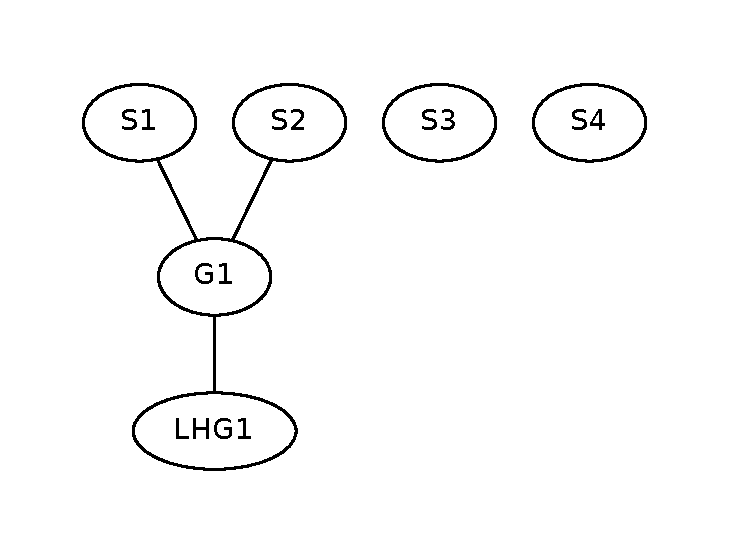
\includegraphics[width=7.0cm]{fig/labgroup/slack_add_1.pdf}        
  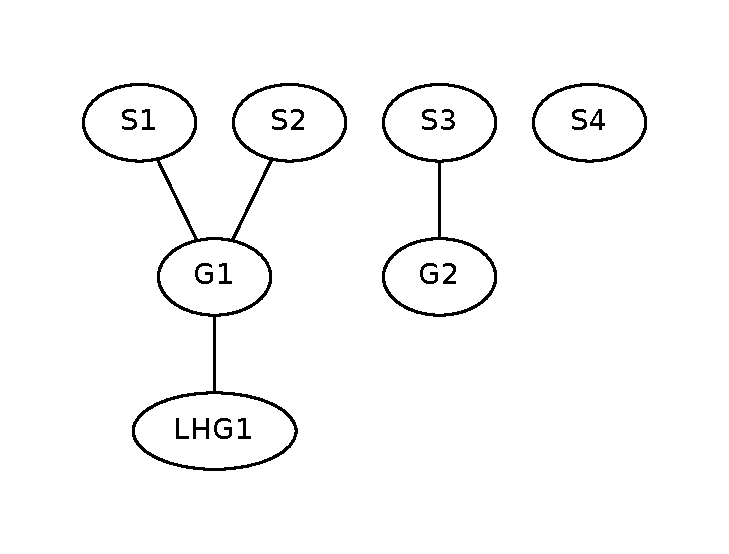
\includegraphics[width=7.0cm]{fig/labgroup/slack_add_2.pdf}        
  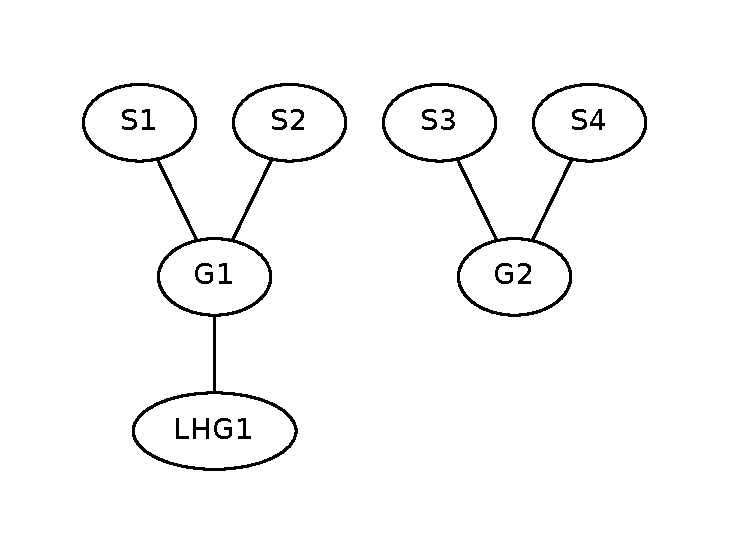
\includegraphics[width=7.0cm]{fig/labgroup/slack_add_2-5.pdf}        
  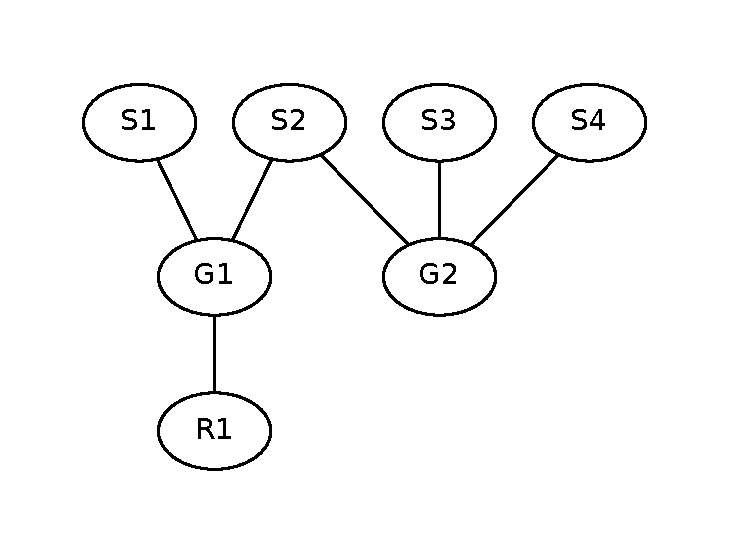
\includegraphics[width=7.0cm]{fig/labgroup/slack_add_3.pdf}        
  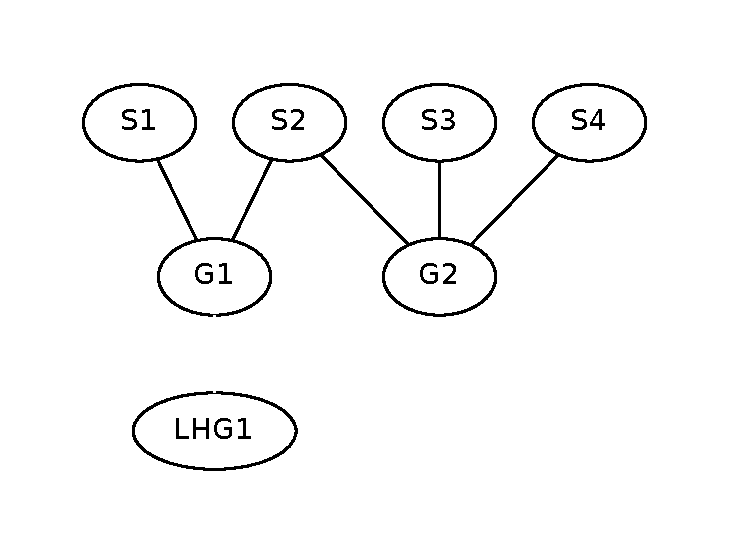
\includegraphics[width=7.0cm]{fig/labgroup/slack_add_4.pdf}        
  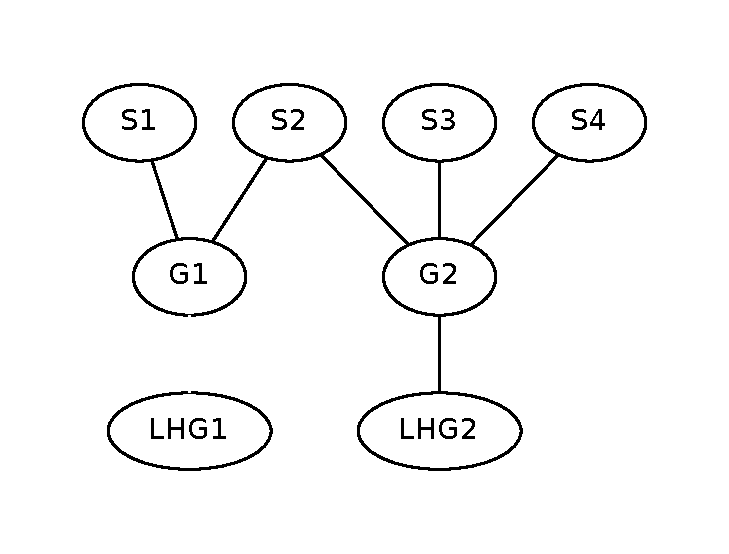
\includegraphics[width=7.0cm]{fig/labgroup/slack_add_5.pdf}        
  \caption[Serie tillstånd rörande labgrupper.]
  {Serie tillstånd rörande labgrupper. Studenterna $S2$, $S3$ och $S4$ vill
  bilda en nya laboraionsgrupp tillsammans (den som blev $G2$) där de ska skapa
  en LHG. Notera hur student $S2$ måste ta bort sin förra LHG innan någon elev
  kan lägga till en LHG i den nya gruppen. Mellan varje figur krävs att någon
  användare gör en åtgärd i waters system.}
  \label{fig:slack_series}
  
\end{figure}

\subsection{Alltid exakt en LHG per laboration ($= 1$)}
Den mindre strikta ($\leq 1$) invarianten ger Water möjligheten att ha ett intuitivt användargränssnitt eftersom ingen student vill se att de gör samma laboration via två olika grupper samtidigt. En striktare variant är dock önskvärd av tekniska skäl. Med en striktare variant behövs till exempel inte hantering av fall då en LHG inte finns, eftersom att den alltid finns. Detta öppnar även upp för att förenkla våra databasförfrågningar, vi kan till exempel få reda på alla laborationer för en student i en kurs genom att “gå” via kopplingarna, eftersom vi har en 1-till-1–relation mellan “laboration-till-grupp”-koppling och laboration per student.

En operationsuppsättning för denna invariant måste även definiera initialtillståndet eftersom det går inte längre att ha studenter utan LHG:s vid kursstart. Operationerna som måste beaktas för denna invariant är fler eftersom tillägg av student eller laboration både är icketriviala. Ifall en student läggs till i en kurs så måste den “direkt” få sina LHG:s. Laborationstillägg måste även se till att varje student får en LHG för den nyligen skapade laborationen. En operation som inte längre kan finnas är att manuellt ta bort en LHG för då skulle invarianten brytas direkt.

\subsubsection{Förslag på implementering}
Invarianten kan  framtvingas genom följande initialtillstånd och operationsuppsättning.

\paragraph{Initialtillstånd}
I början är alla studenter inplacerade i en för varje student unik grupp som kallas “studentens grupp” (förkortat SG i figurerna). Varje student har en sådan grupp som innehåller en LHG till alla laborationer som finns registrerade i kursen. Se figur \ref{fig:strict-initstate}.

\begin{figure}
  \centering
  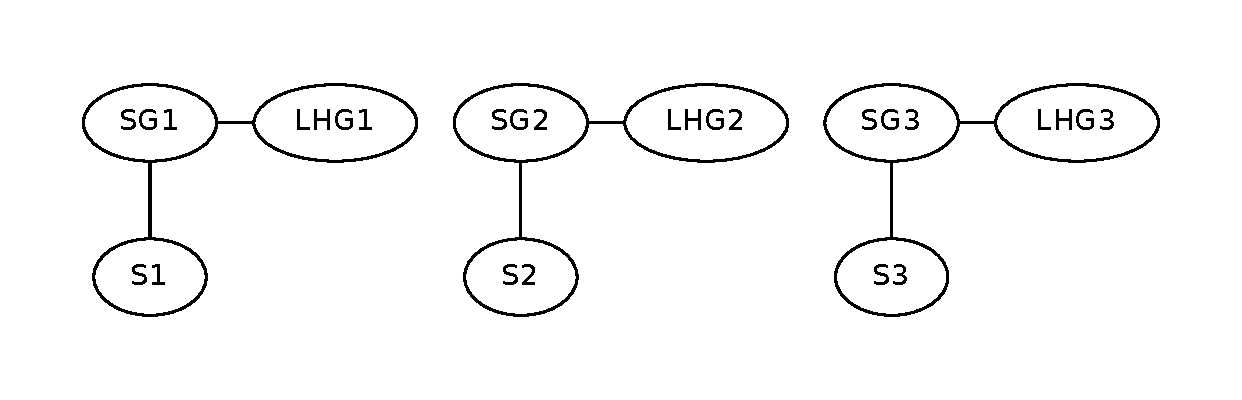
\includegraphics[width=8.0cm]{fig/labgroup/strict_initstate.pdf}
  \caption{Illustration av initialtillståndet i en kurs med 3 studenter}\label{fig:strict-initstate}
\end{figure}

\paragraph{Operationer}
I detta förslag behandlas operationerna “skapa en grupp” och “lägg till en student i gruppen” på samma sätt som i förslaget för den mindre strika invarianten. Att skapa en ny LHG kommer inte ha kräva några förhandsvilkor, studenten behöver alltså inte längre manuellt se till så att LHG:en sätts in genom att ta bort sina egna kopplingar i sina tidigare grupper, istället tar Water bort alla kopplingar som “är i vägen”. Operationen sker mer specifikt på följande sätt:
\begin{enumerate}
  \item För alla medlemmar i gruppen där LHG:en ska läggas till måste deras LHG för den labroationen tas bort.  (De har redan exakt en sådan på grund av invarianten.)
  \item Lägg till LHG:en, nu skall invarianten stämma för gruppmedlemmarna.
  \item Lägg till LHG:en, nu skall invarianten stämma för gruppmedlemmarna.
  \item Borttagningarna i steg ulterkan ha påverkae studenter i andra grupper (FIXA referens se bild). nt påverkade studenterna lägger vi till en LHG i deras egna  tudents laborationsgrupp. De påverkade studenterna kallas för “laborationskamraternas laborationskamrater”. 
\end{enumerate}

Notera att ovanstånde deloperationer sker atomärt, alltså ingenting sker mellan stegen, detta eftersom invarianten blir bruten mellan deloperationerna.

Då en student läggs till en kurs skapas en LHG för varje laboration som placeras i studentens grupp. Då en ny laboration skapas för en kurs så kommer varje student få en LHG för den laborationen insatt i sin egna grupp.

\begin{proof}[Bevis av korrekthet]
I initialtillståndet är invarianten uppenbarligen uppfylld, samt även efter tillägg av student eller laboration. Den enda kvarstående operationen är skapande av en LHG vars beskrivning delats upp i 3 deloperationer. 

Låt mängden A (se figur \ref{fig:strict-proof}) vara samtliga involverade elever som påverkas av operationen, alltså studenten som aktivt lägger till LHG:en, laborationskamraterna till den eleven samt laborationskamraternas laborationskamrater som får sin LHG borttagen i steg 1. 

Låt mängden B vara de elever som är med i laborationsgruppen där LHG:en skapas i steg 2, notera alltså att B$\subseteq$A, notera även att de elever som berörs i steg 3 är A$\setminus$B.

I början antags invarianten vara uppfylld, efter steg 1 så har studenterna i A ingen LHG, efter steg 2 har eleverna i B en ny LHG, endast A$\setminus$B saknar var sin LHG nu, vilket steg 3 åtgärdar. \qedhere
\end{proof}
 
\begin{figure}
  \centering
  \begin{subfigure}[b]{0.5\textwidth}
    \centering
    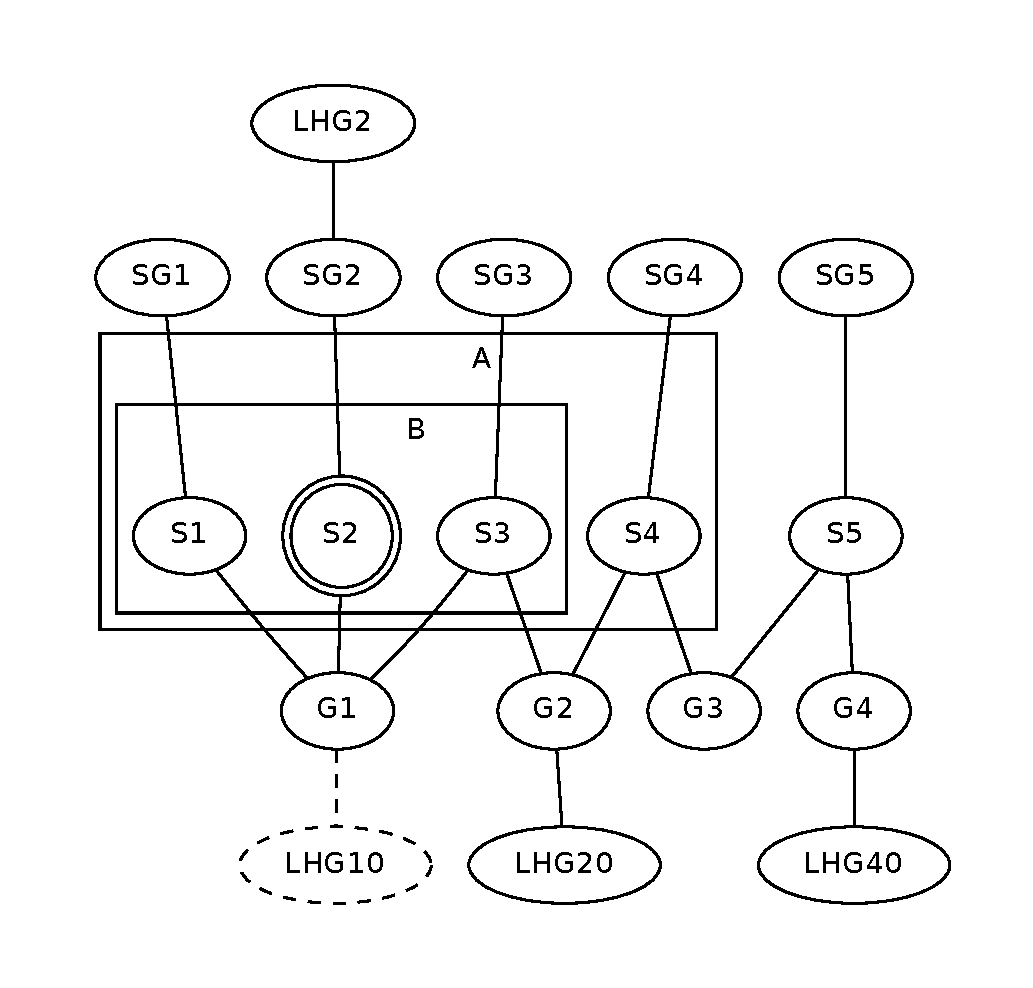
\includegraphics[width=8.0cm]{fig/labgroup/strict_proof.pdf}
    \caption{Situation när $S3$ ska lägga till $R20$}
    \label{fig:strict-proof}
  \end{subfigure}%
        ~ %add desired spacing between images, e. g. ~, \quad, \qquad etc. 
          %(or a blank line to force the subfigure onto a new line)
  \begin{subfigure}[b]{0.5\textwidth}
    \centering
    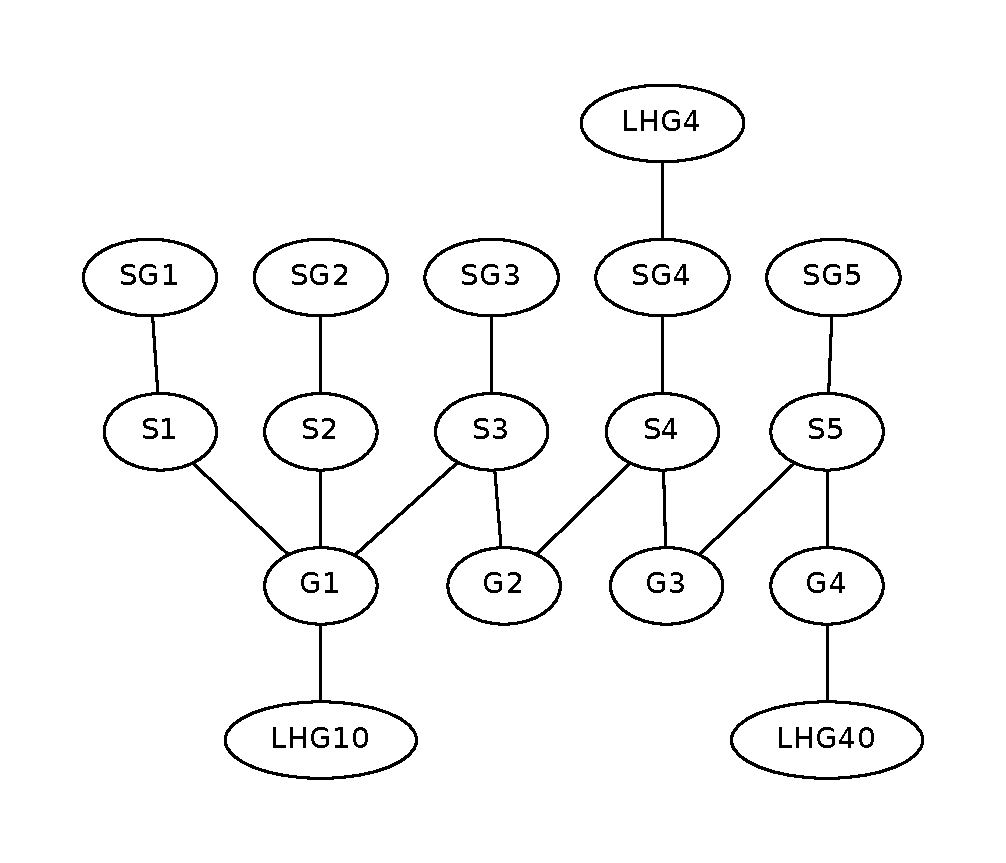
\includegraphics[width=8.0cm]{fig/labgroup/strict_proof_continue.pdf}
    \caption{Situation efter $R20$ lagts till}
    \label{fig:strict-proof-continue}
  \end{subfigure}
  \caption{Före och efter LHG-tillägg (strikt invariant)}\label{fig:animals}
\end{figure}

\subsubsection{Användarperspektiv}
Det ovanstående sättet att skapa en ny LHG innebär att även laborationskamraternas laborationskamrater påverkas av den aktiva studentens operation (se figur \ref{fig:strict-proof-continue}). Detta är givetvis inte bra för de utsatta studenterna. Att samtliga studenter har en egen laborationsgrupp kan vara förvirrande för användare som ser att de redan är medlemmar i en laborationsgrupp som är låst och redan har påbörjat sina laborationer. I gengäld kräver operationen färre steg för en student att påbörja en laboration med en annan laborationsgrupp.

\subsection{Ingen invaraint}
Naturligtvis går det att strunta i att forcera någon invariant. Det blir minimalt med jobb och ingenting behöver bevisas. Nackdelen är att det lätt blir förvirrande för användaren att ha flera aktiva laborationer samtidigt. Vidare krävs fler användaroperationer för att lokalisera sin LHG då användaren inte bara behöver specifiera laboration utan även laborationsgrupp.

\begin{flushright}
  
  \textbf{Beslut}
  
  Vi valde att implementera ($\leq 1$) invarianten. Vi satte hög prestige i ett interface där användare direkt kan klicka på deras laboration utan att först välja laborationsgrupp.
\end{flushright}

\section{Statistik}

Att ha tillgång till statistik från tidigare år hjälper examinatorer att successivt utforma innehållet av laborationer. Till exempel kan en laboration vara för omfattande och då ta för lång tid, vilket resulterar i att de flesta inlämingar kommer in sent, eller inte alls. Det kan också vara av intresse för examinatorn att se hur stor andel av studenterna klarade av en viss laboration.  

Detta kan tas fram genom att implementera attribut i databasen, med vilka statistiken kan tas fram, till exempel ett attribut som innehåller tidpunkten då en grupp gjorde en inlämning.

Datan kan sammaställas i en tabell, med vilken man lätt kan jämföra olika årgångar.

\section{Plagiatkontroll}
På Chalmers upprätthålls den akademiska hederligheten. För inlämningsuppgifter, speciellt programmeringsuppgifter, är det vanligt förekommande att man får samarbeta i någon form. Beroende på inlämningsuppgiftens instruktioner är det ibland godkänt att samarbeta mellan grupper, medan det ibland är av vikt att gruppen lämnar in en unik lösning. (Chalmers tekniska högskola, 2009) I det senare fallet kan det vara tillhanda att automatiskt plagiatkontroll implementeras i inlämningssystemet.

Urkund är ett system för automatisk plagiatkontroll. Texter som behandlas av Urkund jämförs med en bred databas som består av tidigare verk. I dagsläget använder lärare sig utav e-post för att skicka material till Urkund vid misstanke om plagiat. Då Urkund erbjuder ett API till sina kunder (URKUND, 2012), skulle denna process kunna göras betydligt smidigare genom att integrera funktionaliteten direkt i Water.

Ytterligare skulle en intern kontroll av tidigare inlämningar kunna implementeras. För att detta skulle vara möjligt måste samtliga inlämningar som laddas upp till Water behöva sparas i databasen. Därefter skulle en lämplig algoritm för filjämförelse behöva implementeras.

\begin{flushright}
  
  \textbf{Beslut}
  
  Plagiatkontroll nedprioriteras och implementeras inte.
  
\end{flushright}
